\documentclass{article}
\usepackage[final]{nips_2017}
\usepackage{polski}
\usepackage[utf8]{inputenc}    % allow utf-8 input
\usepackage[T1]{fontenc}       % use 8-bit T1 fonts
\usepackage{hyperref}          % hyperlinks
\usepackage{url}               % simple URL typesetting
\usepackage{booktabs}          % professional-quality tables
\usepackage{amsfonts}          % blackboard math symbols
\usepackage{nicefrac}          % compact symbols for 1/2, etc.
\usepackage{microtype}         % microtypography
\usepackage[section]{placeins} % figures kept in sections
\usepackage{graphicx}          % images
\graphicspath{ {./img/} }
\usepackage{multirow}
\usepackage{float}             % figures in place
\usepackage{caption}		   % smaller margin after figure

\renewcommand{\figurename}{Wykres}
\setlength{\belowcaptionskip}{-20pt}

\title{  Optymalizacja uczenia\\Sieci Neuronowe 2020 }

\author{
  Jakub Ciszek \\
  238035\\
}

\begin{document}

\maketitle

\newpage
\tableofcontents
\newpage

Cały kod wykorzystany w zadaniu znajduje się pod adresem: \url{https://github.com/Greenpp/sieci-neuronowe-pwr-2020}

\section{Opis badań}
\subsection{Plan eksperymentów}

Wszystkie eksperymenty zostały przeprowadzone 10 razy. Losowość przy inicjalizacji wag oraz generacji danych nie została narzucona żadnym ziarnem. Podczas badań przyjęto górną granicę 5 epok, po przekroczeniu której, uczenie zostawało przerywane. Ze względu na charakter zadania (klasyfikacja) na ostatniej warstwie użyto funkcji Softmax, a za funkcję straty przyjęto Entropię krzyżową. Warstwa ukryta składała się z 512 neuronów, a początkowy współczynnik uczenia wynosił 0.01.
Z powodów wydajnościowych testowanie modelu przeprowadzano co każde 32 paczki, z których każda składała się z 32 przykładów.\\
Zgodnie z instrukcją zostały przeprowadzone następujące badania:
\begin{itemize}
	\item Wpływ optymalizatorów na przebieg procesu uczenia
	\item Wpływ inicjalizacji wag na przebieg procesu uczenia 
\end{itemize}
Podczas wizualizacji funkcji straty pominięto pierwsze 10 pomiarów dla lepszej czytelności.

\subsection{Charakterystyka zbiorów danych}

Danymi użytymi w zadaniu jest zbiór ręcznie pisanych cyfr \(0-9\) - MNIST. Na zbiór składa się 70,000 obrazów wielkości 28x28 pikseli, co po przekształceniu odpowiadało 784 elementowemu wektorowi wejściowemu i 10 klasom na wyjściu. Użyta w zadaniu wersja została podzielona na 3 zbiory:
\begin{itemize}
	\item Uczący - 50,000 przykładów.
	\item Walidujący - 10,000 przykładów.
	\item Testowy - 10,000 przykładów.
\end{itemize}
W trakcie eksperymentów wykorzystano jedynie zbiory uczący i testowy.

\newpage
\section{Eksperymenty}

\subsection{Wpływ optymalizatorów na przebieg procesu uczenia}
\subsubsection*{Założenia}
\begin{table}[H]
	\caption{Stałe dla eksperymentu 1}
	\label{tabela-const-1}
	\centering
	\begin{tabular}{lr}
		\toprule
		Parametr          & Wartość         \\
		\midrule
		Inicjalizacja wag & \($-0.1 -- 0.1$\) \\
		\bottomrule
	\end{tabular}
\end{table}

Zmienną w tym eksperymencie był użyty optymalizator uczenia. Użyto metod ze zbioru \(\{$SGD, Momentum, Nesterov, AdaGrad, AdaDelta, Adam$\}\)
\subsubsection*{Przebieg}

Podczas eksperymentu model został zainicjalizowany 10 razy dla każdej z badanych wartości oraz wyuczony, uzyskane wyniki zostały zapisane w postaci pliku .plk do dalszej analizy. Badania wykonano dla funkcji aktywacji Sigmoid oraz ReLU.

\subsubsection*{Wyniki}
\begin{figure}[H]
	\centering
	\caption{Dokładność modelu w zależności od użytego optymalizatora dla funkcji ReLU}
	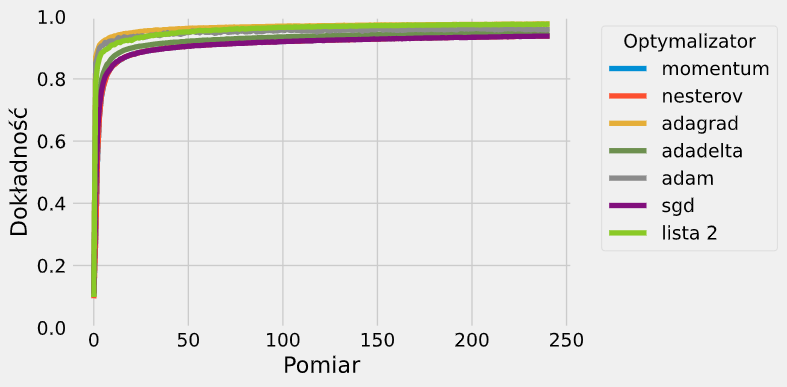
\includegraphics[width=\textwidth]{opt_relu_acc.png}
	\label{fig:res101}
\end{figure}
\begin{figure}[H]
	\centering
	\caption{Dokładność modelu w końcowym etapie uczenia w zależności od użytego optymalizatora dla funkcji ReLU}
	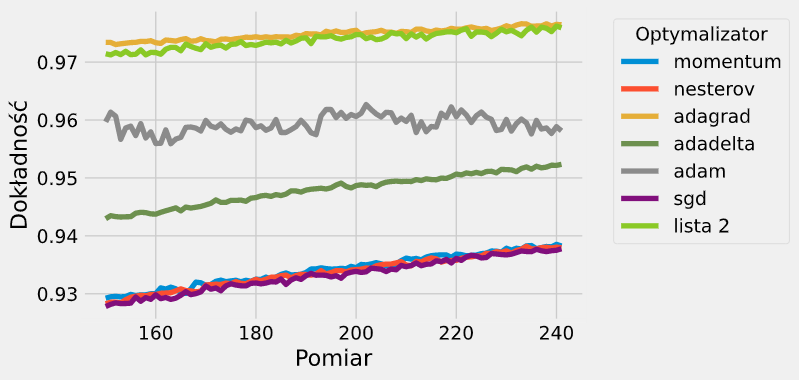
\includegraphics[width=\textwidth]{opt_relu_acc_zoom.png}
	\label{fig:res102}
\end{figure}
\begin{figure}[H]
	\centering
	\caption{Zachowanie funkcji błędu dla funkcji ReLU i optymalizatora Momentum}
	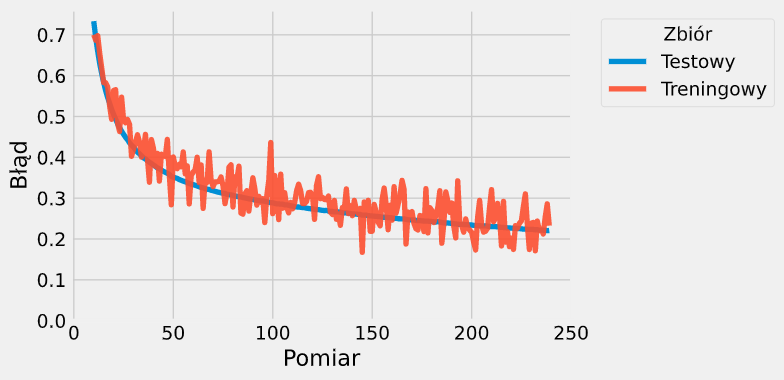
\includegraphics[width=\textwidth]{relu_mom_err.png}
	\label{fig:res103}
\end{figure}
\begin{figure}[H]
	\centering
	\caption{Zachowanie funkcji błędu dla funkcji ReLU i optymalizatora Nesterov}
	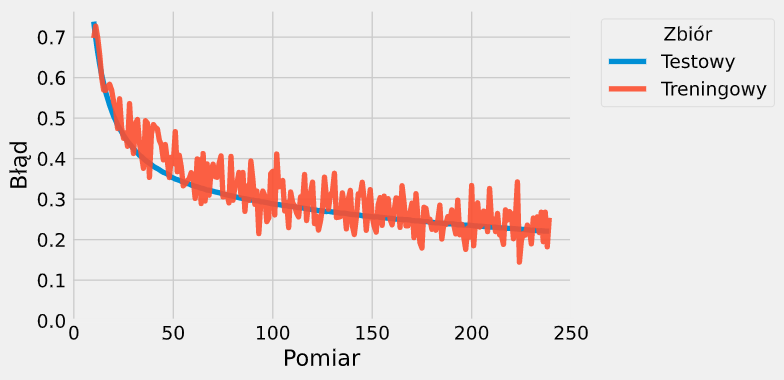
\includegraphics[width=\textwidth]{relu_nes_err.png}
	\label{fig:res104}
\end{figure}
\begin{figure}[H]
	\centering
	\caption{Zachowanie funkcji błędu dla funkcji ReLU i optymalizatora AdaGrad}
	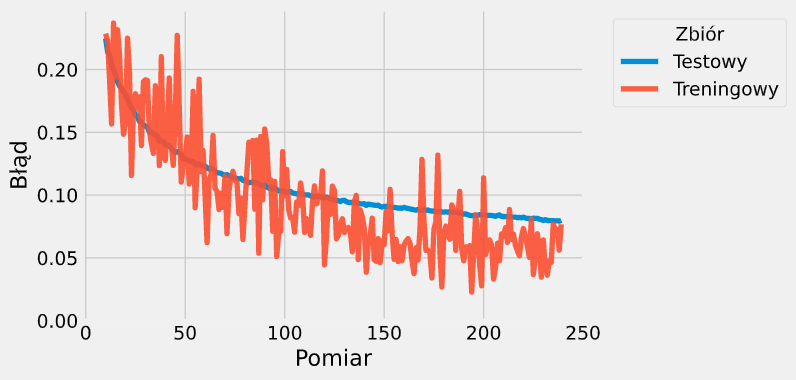
\includegraphics[width=\textwidth]{relu_grad_err.png}
	\label{fig:res105}
\end{figure}
\begin{figure}[H]
	\centering
	\caption{Zachowanie funkcji błędu dla funkcji ReLU i optymalizatora AdaDelta}
	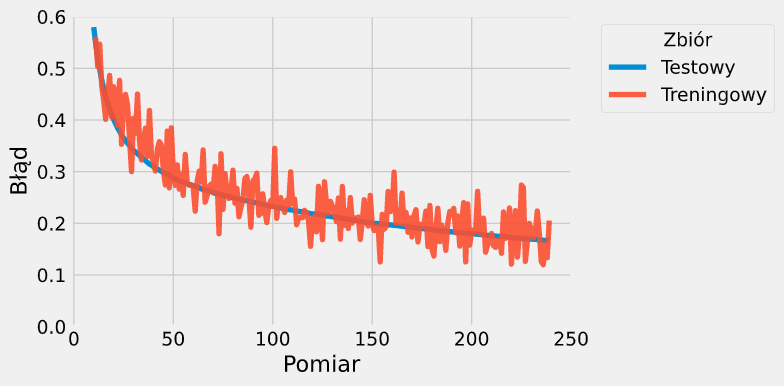
\includegraphics[width=\textwidth]{relu_delta_err.png}
	\label{fig:res106}
\end{figure}
\begin{figure}[H]
	\centering
	\caption{Zachowanie funkcji błędu dla funkcji ReLU i optymalizatora Adam}
	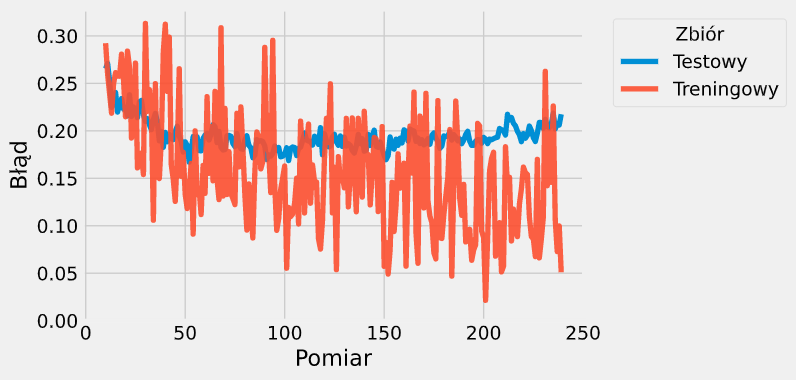
\includegraphics[width=\textwidth]{relu_adam_err.png}
	\label{fig:res107}
\end{figure}
\begin{figure}[H]
	\centering
	\caption{Zachowanie funkcji błędu dla funkcji ReLU i optymalizatora SGD}
	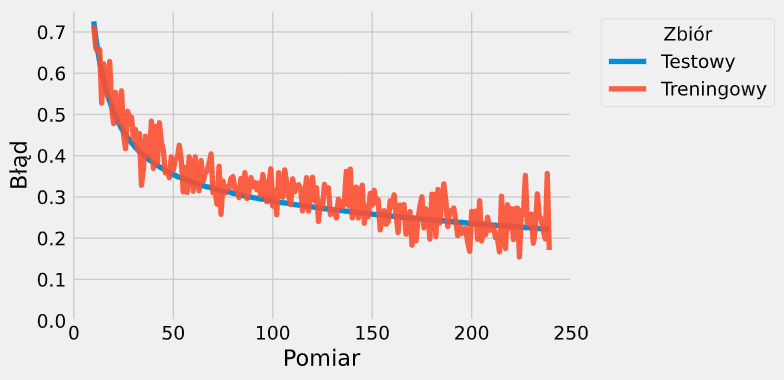
\includegraphics[width=\textwidth]{relu_sgd_err.png}
	\label{fig:res108}
\end{figure}
\begin{figure}[H]
	\centering
	\caption{Zachowanie funkcji błędu dla funkcji ReLU z listy 2}
	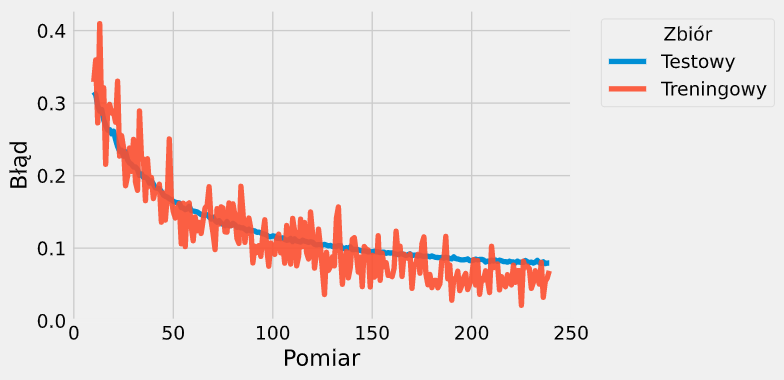
\includegraphics[width=\textwidth]{relu_2_err.png}
	\label{fig:res109}
\end{figure}
\begin{figure}[H]
	\centering
	\caption{Dokładność modelu w zależności od użytego optymalizatora dla funkcji Sigmoid}
	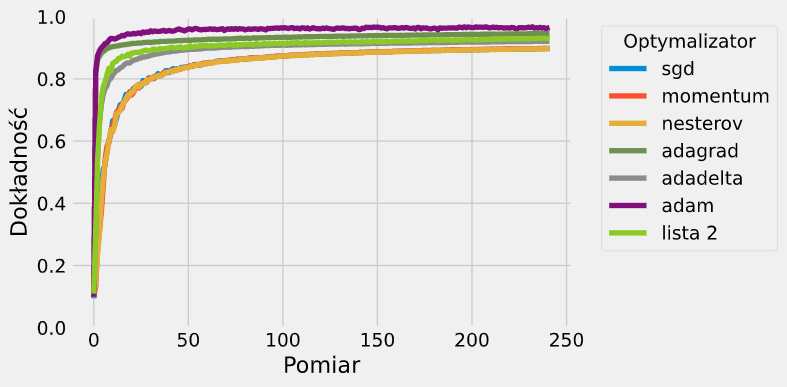
\includegraphics[width=\textwidth]{opt_sig_acc.png}
	\label{fig:res110}
\end{figure}
\begin{figure}[H]
	\centering
	\caption{Dokładność modelu w końcowym etapie uczenia w zależności od użytego optymalizatora dla funkcji Sigmoid}
	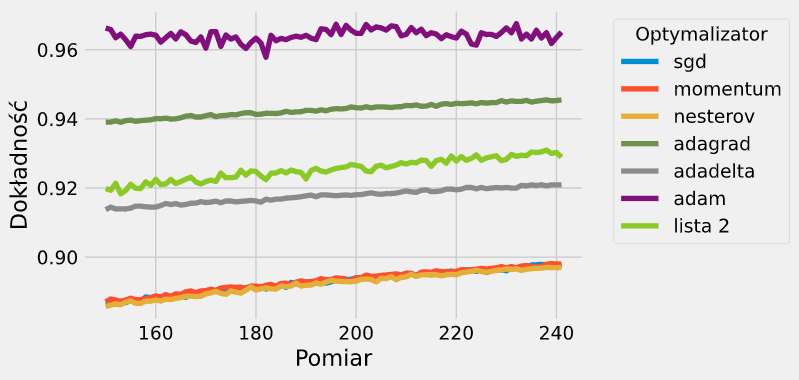
\includegraphics[width=\textwidth]{opt_sig_acc_zoom.png}
	\label{fig:res111}
\end{figure}
\begin{figure}[H]
	\centering
	\caption{Zachowanie funkcji błędu dla funkcji Sigmoid i optymalizatora Momentum}
	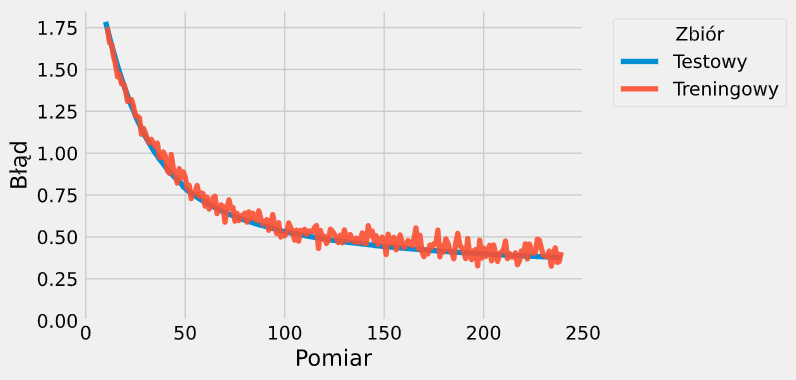
\includegraphics[width=\textwidth]{sig_mom_err.png}
	\label{fig:res112}
\end{figure}
\begin{figure}[H]
	\centering
	\caption{Zachowanie funkcji błędu dla funkcji Sigmoid i optymalizatora Nesterov}
	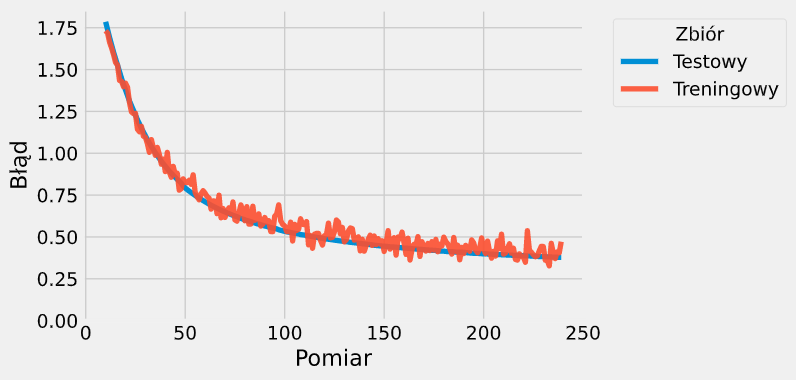
\includegraphics[width=\textwidth]{sig_nes_err.png}
	\label{fig:res113}
\end{figure}
\begin{figure}[H]
	\centering
	\caption{Zachowanie funkcji błędu dla funkcji Sigmoid i optymalizatora AdaGrad}
	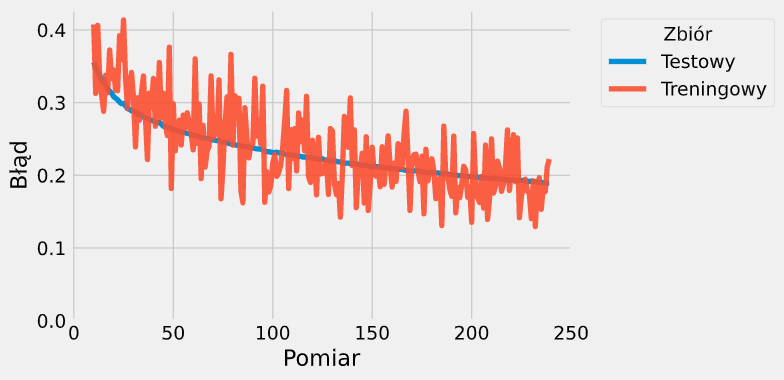
\includegraphics[width=\textwidth]{sig_grad_err.png}
	\label{fig:res114}
\end{figure}
\begin{figure}[H]
	\centering
	\caption{Zachowanie funkcji błędu dla funkcji Sigmoid i optymalizatora AdaDelta}
	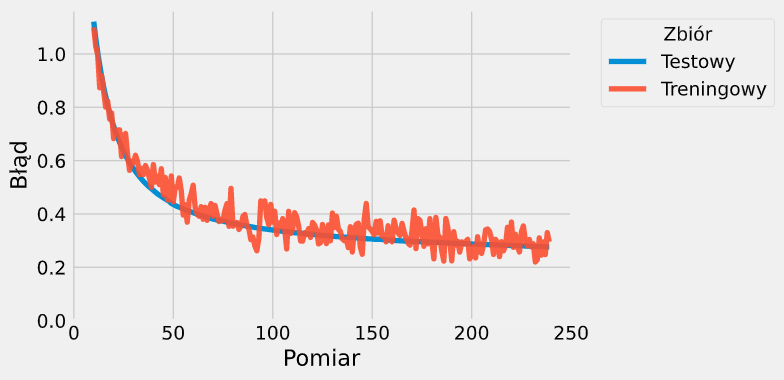
\includegraphics[width=\textwidth]{sig_delta_err.png}
	\label{fig:res115}
\end{figure}
\begin{figure}[H]
	\centering
	\caption{Zachowanie funkcji błędu dla funkcji Sigmoid i optymalizatora Adam}
	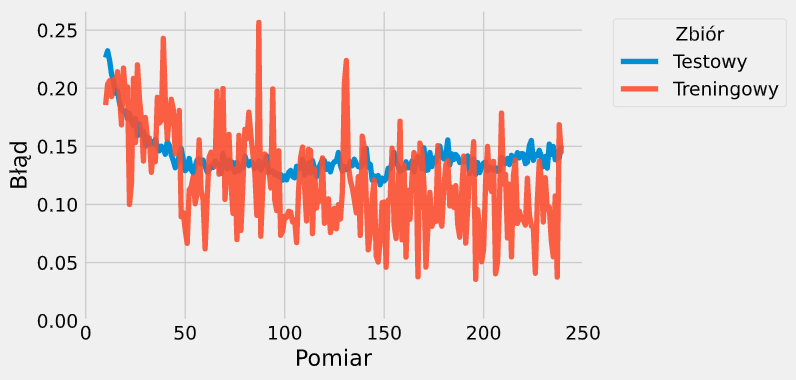
\includegraphics[width=\textwidth]{sig_adam_err.png}
	\label{fig:res116}
\end{figure}
\begin{figure}[H]
	\centering
	\caption{Zachowanie funkcji błędu dla funkcji Sigmoid i optymalizatora SGD}
	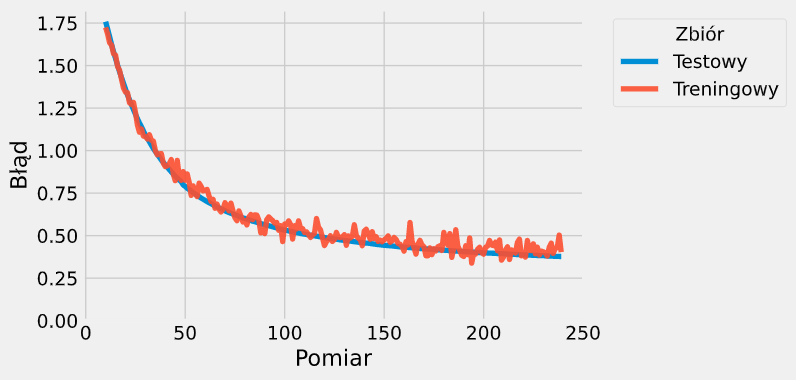
\includegraphics[width=\textwidth]{sig_sgd_err.png}
	\label{fig:res117}
\end{figure}
\begin{figure}[H]
	\centering
	\caption{Zachowanie funkcji błędu dla funkcji Sigmoid z listy 2}
	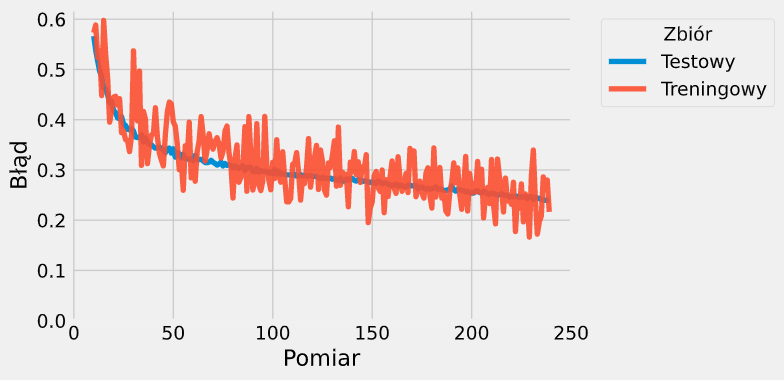
\includegraphics[width=\textwidth]{sig_2_err.png}
	\label{fig:res118}
\end{figure}

\begin{table}[H]
	\caption{Średnia maksymalna dokładność w zależności od użytego optymalizatora}
	\label{tabela-res-11}
	\centering
	\begin{tabular}{rrr}
		\toprule
		\multirow{2}{*}{Optymalizator} & \multicolumn{2}{c}{Dokładność [\%]} \\
		         & ReLU           & Sigmoid        \\
		\midrule
		Momentum & 93.92          & 89.91          \\
		Nesterov & 93.91          & 89.81          \\
		AdaGrad  & \textbf{97.72} & 94.62          \\
		AdaDelta & 95.28          & 92.21          \\
		Adam     & 93.86          & \textbf{97.15} \\
		SGD      & 93.86          & 89.89          \\
		Lista 2  & 97.70          & 93.29          \\
		\bottomrule
	\end{tabular}
\end{table}

\subsubsection*{Wnioski}
Na przedstawionych wykresach~\ref{fig:res101},~\ref{fig:res102} oraz tabeli~\ref{tabela-res-11} można zauważyć, że najlepszym wyborem przy użyciu funkcji ReLU był optymalizator AdaGrad, kolejne miejsce osiągnął Adam. Patrząc dodatkowo na wykresy~\ref{fig:res110} i~\ref{fig:res111}, widać, że dla funkcji Sigmoid sytuacja jest odwrotna, najlepszy wynik otrzymują modele uczone metodą Adam, a AdaGrad jest na drugim miejscu. Powodem prowadzenia tych metod może być widoczna na wykresach~\ref{fig:res103} -~\ref{fig:res109} i~\ref{fig:res112} -~\ref{fig:res118} większa niestabilność błędu treningowego dla tych metod, co może oznaczać lepszą eksplorację minimów lokalnych. Porównując jednak funkcje błędu metod Adam i AdaGrad widać, że w przypadku optymalizatora Adam błąd testowy w pewnym momencie zaczyna rosnąć, co może wskazywać przeuczenie. Nie jest to jednak problemem na zbiorze MNIST. W porównaniu z modelem otrzymanym w poprzednim zadaniu konfiguracja z funkcją ReLU przy użyciu metody AdaGrad daje bardzo zbliżone wyniki, jednak AdaGrad ma przewagę w początkowym etapie uczenia gdzie szybciej osiąga wysoką dokładność, na co wpływa dynamiczny współczynnik dla każdej z wag. W przypadku modelu z funkcją Sigmoidalną, poprzedni model znajduje się dopiero na 3 miejscu, spowodowane jest to najprawdopodobniej dobraniem w poprzednim zadaniu hiperparametrów dla najlepszego wyniku z funkcją ReLU. 

\newpage
\subsection{Wpływ inicjalizacji wag na przebieg procesu uczenia}
\subsubsection*{Założenia}
\begin{table}[H]
	\caption{Stałe dla eksperymentu 2}
	\label{tabela-const-2}
	\centering
	\begin{tabular}{lr}
		\toprule
		Parametr      & Wartość \\
		\midrule
		Optymalizator & SGD       \\
		\bottomrule
	\end{tabular}
\end{table}

Zmienną w tym eksperymencie był sposób inicjalizacji wag. Użyto metod ze zbioru \(\{$Zakres, Xavier, He$\}\). Zakres, z którego losowane były wagi to \($-0.1 -- 0.1$\).
\subsubsection*{Przebieg}

Podczas eksperymentu model został zainicjalizowany 10 razy dla każdej z badanych wartości oraz wyuczony, uzyskane wyniki zostały zapisane w postaci pliku .plk do dalszej analizy. Badania wykonano dla funkcji aktywacji Sigmoid oraz ReLU.

\subsubsection*{Wyniki}
\begin{figure}[H]
	\centering
	\caption{Dokładność modelu w zależności od sposóbu inicjalizacji wag dla funkcji ReLU}
	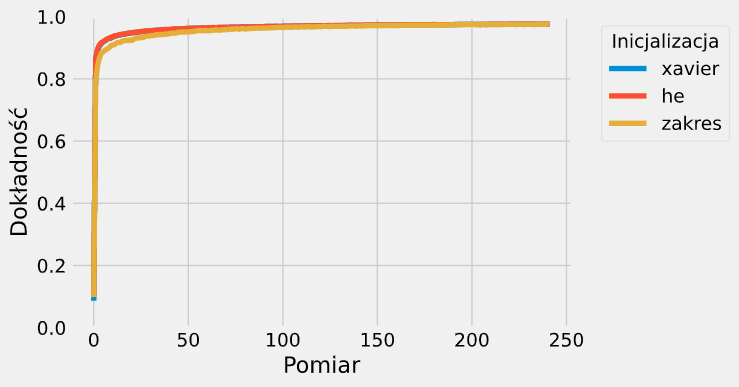
\includegraphics[width=\textwidth]{relu_init_acc.png}
	\label{fig:res201}
\end{figure}
\begin{figure}[H]
	\centering
	\caption{Dokładność modelu w końcowym etapie uczenia w zależności od sposóbu inicjalizacji wag dla funkcji ReLU}
	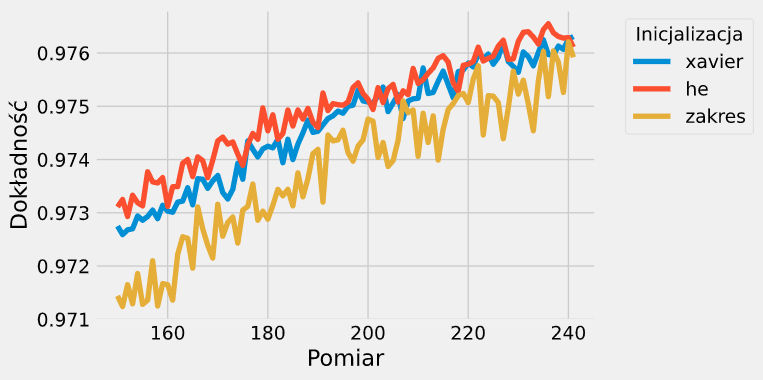
\includegraphics[width=\textwidth]{relu_init_acc_zoom.png}
	\label{fig:res202}
\end{figure}
\begin{figure}[H]
	\centering
	\caption{Zachowanie funkcji błędu dla funkcji ReLU i inicjalizacji z zakresu}
	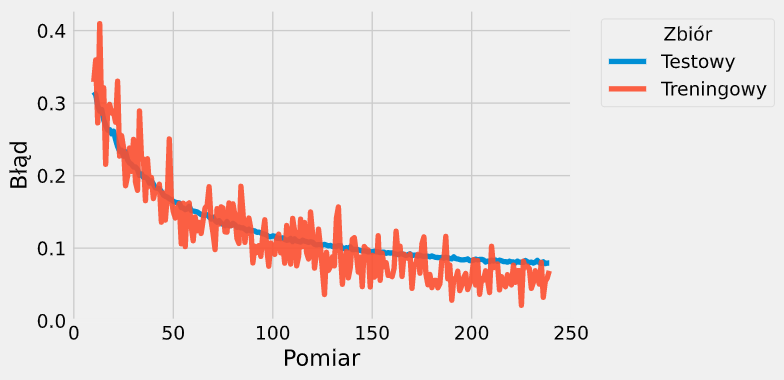
\includegraphics[width=\textwidth]{relu_init_zak.png}
	\label{fig:res203}
\end{figure}
\begin{figure}[H]
	\centering
	\caption{Zachowanie funkcji błędu dla funkcji ReLU i inicjalizacji Xaviera}
	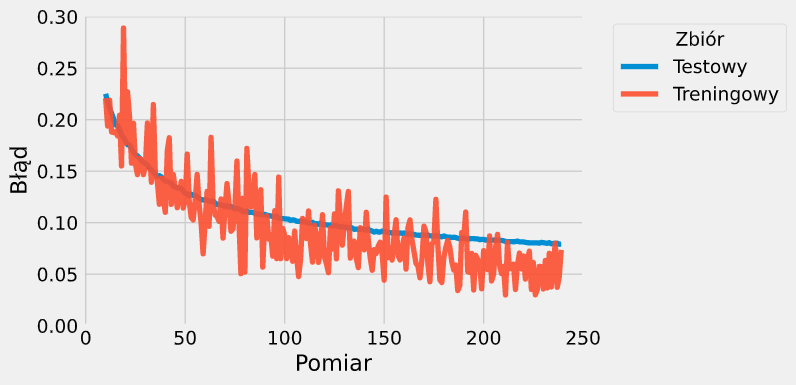
\includegraphics[width=\textwidth]{relu_init_xav.png}
	\label{fig:res204}
\end{figure}
\begin{figure}[H]
	\centering
	\caption{Zachowanie funkcji błędu dla funkcji ReLU i inicjalizacji He}
	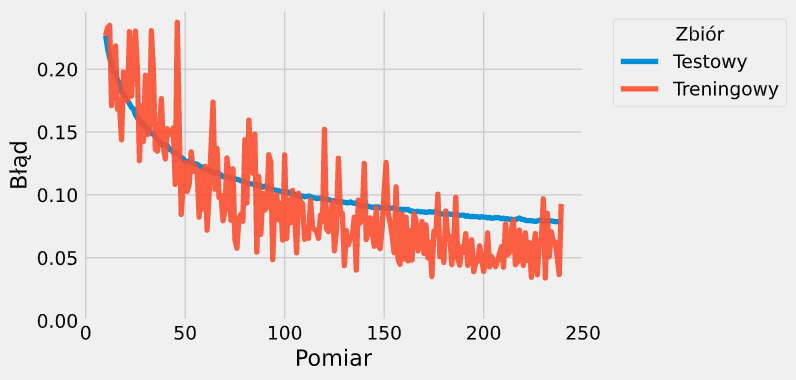
\includegraphics[width=\textwidth]{relu_init_he.png}
	\label{fig:res205}
\end{figure}
\begin{figure}[H]
	\centering
	\caption{Dokładność modelu w zależności od sposóbu inicjalizacji wag dla funkcji Sigmoid}
	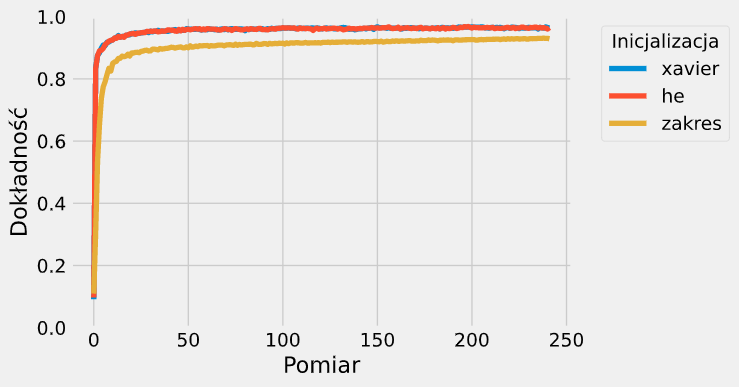
\includegraphics[width=\textwidth]{sig_init_acc.png}
	\label{fig:res206}
\end{figure}
\begin{figure}[H]
	\centering
	\caption{Dokładność modelu w końcowym etapie uczenia w zależności od sposóbu inicjalizacji wag dla funkcji Sigmoid}
	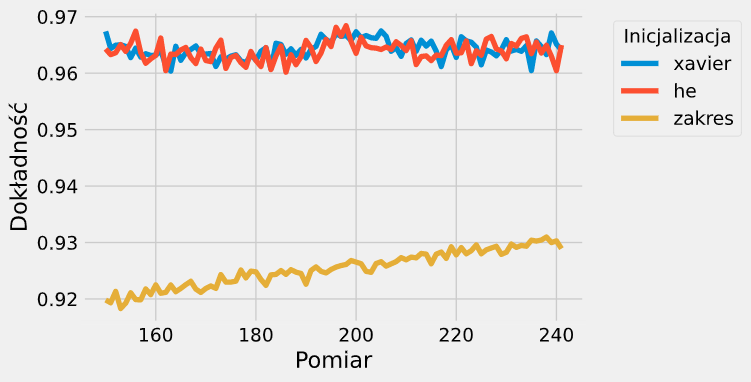
\includegraphics[width=\textwidth]{sig_init_acc_zoom.png}
	\label{fig:res207}
\end{figure}
\begin{figure}[H]
	\centering
	\caption{Zachowanie funkcji błędu dla funkcji Sigmoid i inicjalizacji z zakresu}
	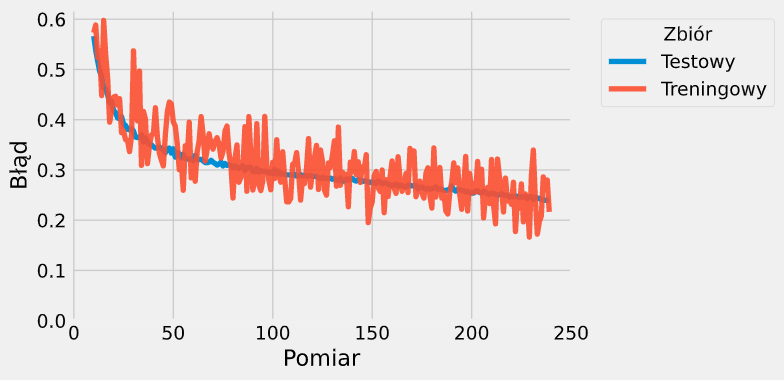
\includegraphics[width=\textwidth]{sig_init_zak.png}
	\label{fig:res208}
\end{figure}
\begin{figure}[H]
	\centering
	\caption{Zachowanie funkcji błędu dla funkcji Sigmoid i inicjalizacji Xaviera}
	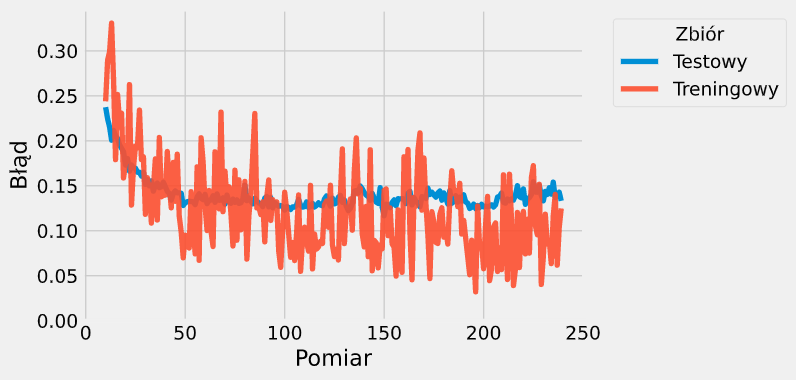
\includegraphics[width=\textwidth]{sig_init_xav.png}
	\label{fig:res209}
\end{figure}
\begin{figure}[H]
	\centering
	\caption{Zachowanie funkcji błędu dla funkcji Sigmoid i inicjalizacji He}
	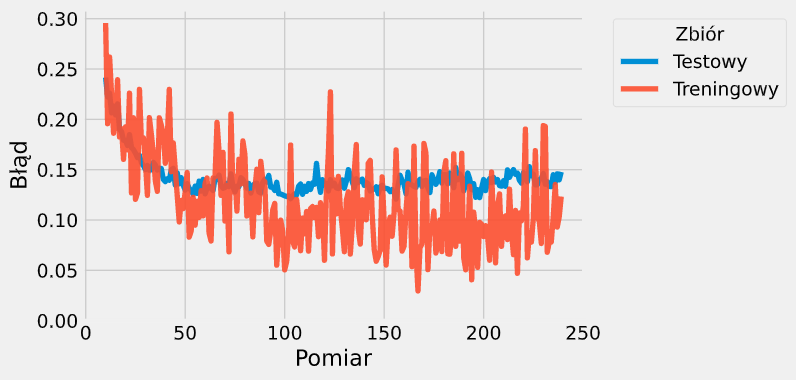
\includegraphics[width=\textwidth]{sig_init_he.png}
	\label{fig:res210}
\end{figure}

\begin{table}[H]
	\caption{Średnia maksymalna dokładność w zależności od sposóbu inicjalizacji wag}
	\label{tabela-res-21}
	\centering
	\begin{tabular}{rrr}
		\toprule
		\multirow{2}{*}{Inicjalizacja} & \multicolumn{2}{c}{Dokładność [\%]} \\
		       & ReLU           & Sigmoid        \\
		\midrule
		Zakres & 97.70          & 93.29          \\
		Xavier & 97.71          & \textbf{97.18} \\
		He     & \textbf{97.73} & 97.16          \\
		\bottomrule
	\end{tabular}
\end{table}

\subsubsection*{Wnioski}

Na przedstawionych wykresach~\ref{fig:res201},~\ref{fig:res202} oraz tabeli~\ref{tabela-res-21} można zauważyć, że dla funkcji ReLU rodzaj inicjalizacji nie miał dużego wpływu. Pomimo różnicy 2 rzędów wielkości pomiędzy inicjalizacjami He (0.0025) i Xaviera (0.0015) a z zakresu (0.1) funkcja ReLU wydaje się być obojętna na wariację wag po przekroczeniu pewnej granicy. Dodając jednak wykresy~\ref{fig:res206} i~\ref{fig:res207} widać, że dla funkcji Sigmoidalnej sytuacja wygląda inaczej. W tym przypadku inicjalizacja He oraz Xaviera dają dużo lepsze wyniki od zakresu. Może to być spowodowane tym, że Sigmoid może operować bez nasycenia tylko w małym przedziale, w przeciwieństwie do ReLU która nie jest ograniczona dla wartości dodatnich. Ponadto na wykresach~\ref{fig:res203}-~\ref{fig:res205} i~\ref{fig:res208}-~\ref{fig:res210} zachowanie funkcji błędu testowego jest znacznie stabilniejsze dla funkcji ReLU, gdzie dla Sigmoida wykazuje symptomy przeuczenia. Jest to jednak najprawdopodobniej wina użytej funkcji, a nie inicjalizacji wag.


\newpage
\section{Wnioski}

\begin{itemize}
	\item Użycie odpowiedniej metody uczenia może przyspieszyć cały proces, a nawet dać lepsze wyniki.
	\item Różne metody dają różne wyniki dla takiego samego początkowego współczynnika uczenia, większość otrzymanych wyników można poprawić dostrajając hiperparametry dla danej metody.
	\item Inicjalizacja wag powinna być przeprowadzana pod użytą funkcję aktywacji.
	\item Dobranie wag w taki sposób aby funkcja aktywacji mogła pracować poza swoimi zakresami nasycenia daje dużo lepsze wyniki.
	\item Różnica pomiędzy inicjalizacjami Xaviera i He nie jest widoczna na małych sieciach.
\end{itemize}

\end{document}